\section{The Waiting Room}\label{chapter:waiting-room}
\textit{In this section we apply the path-space framework developed in Section \ref{chapter:telegraph} to the `waiting room' system as described below. We obtain a closed form for the steady-state entropy production of this non-Markov process. This is the first instance of such a result for a non-Markov system.} 
\subsection{The System}



\begin{figure}
  \begin{subfigure}[b]{0.49\textwidth}
  \centering
  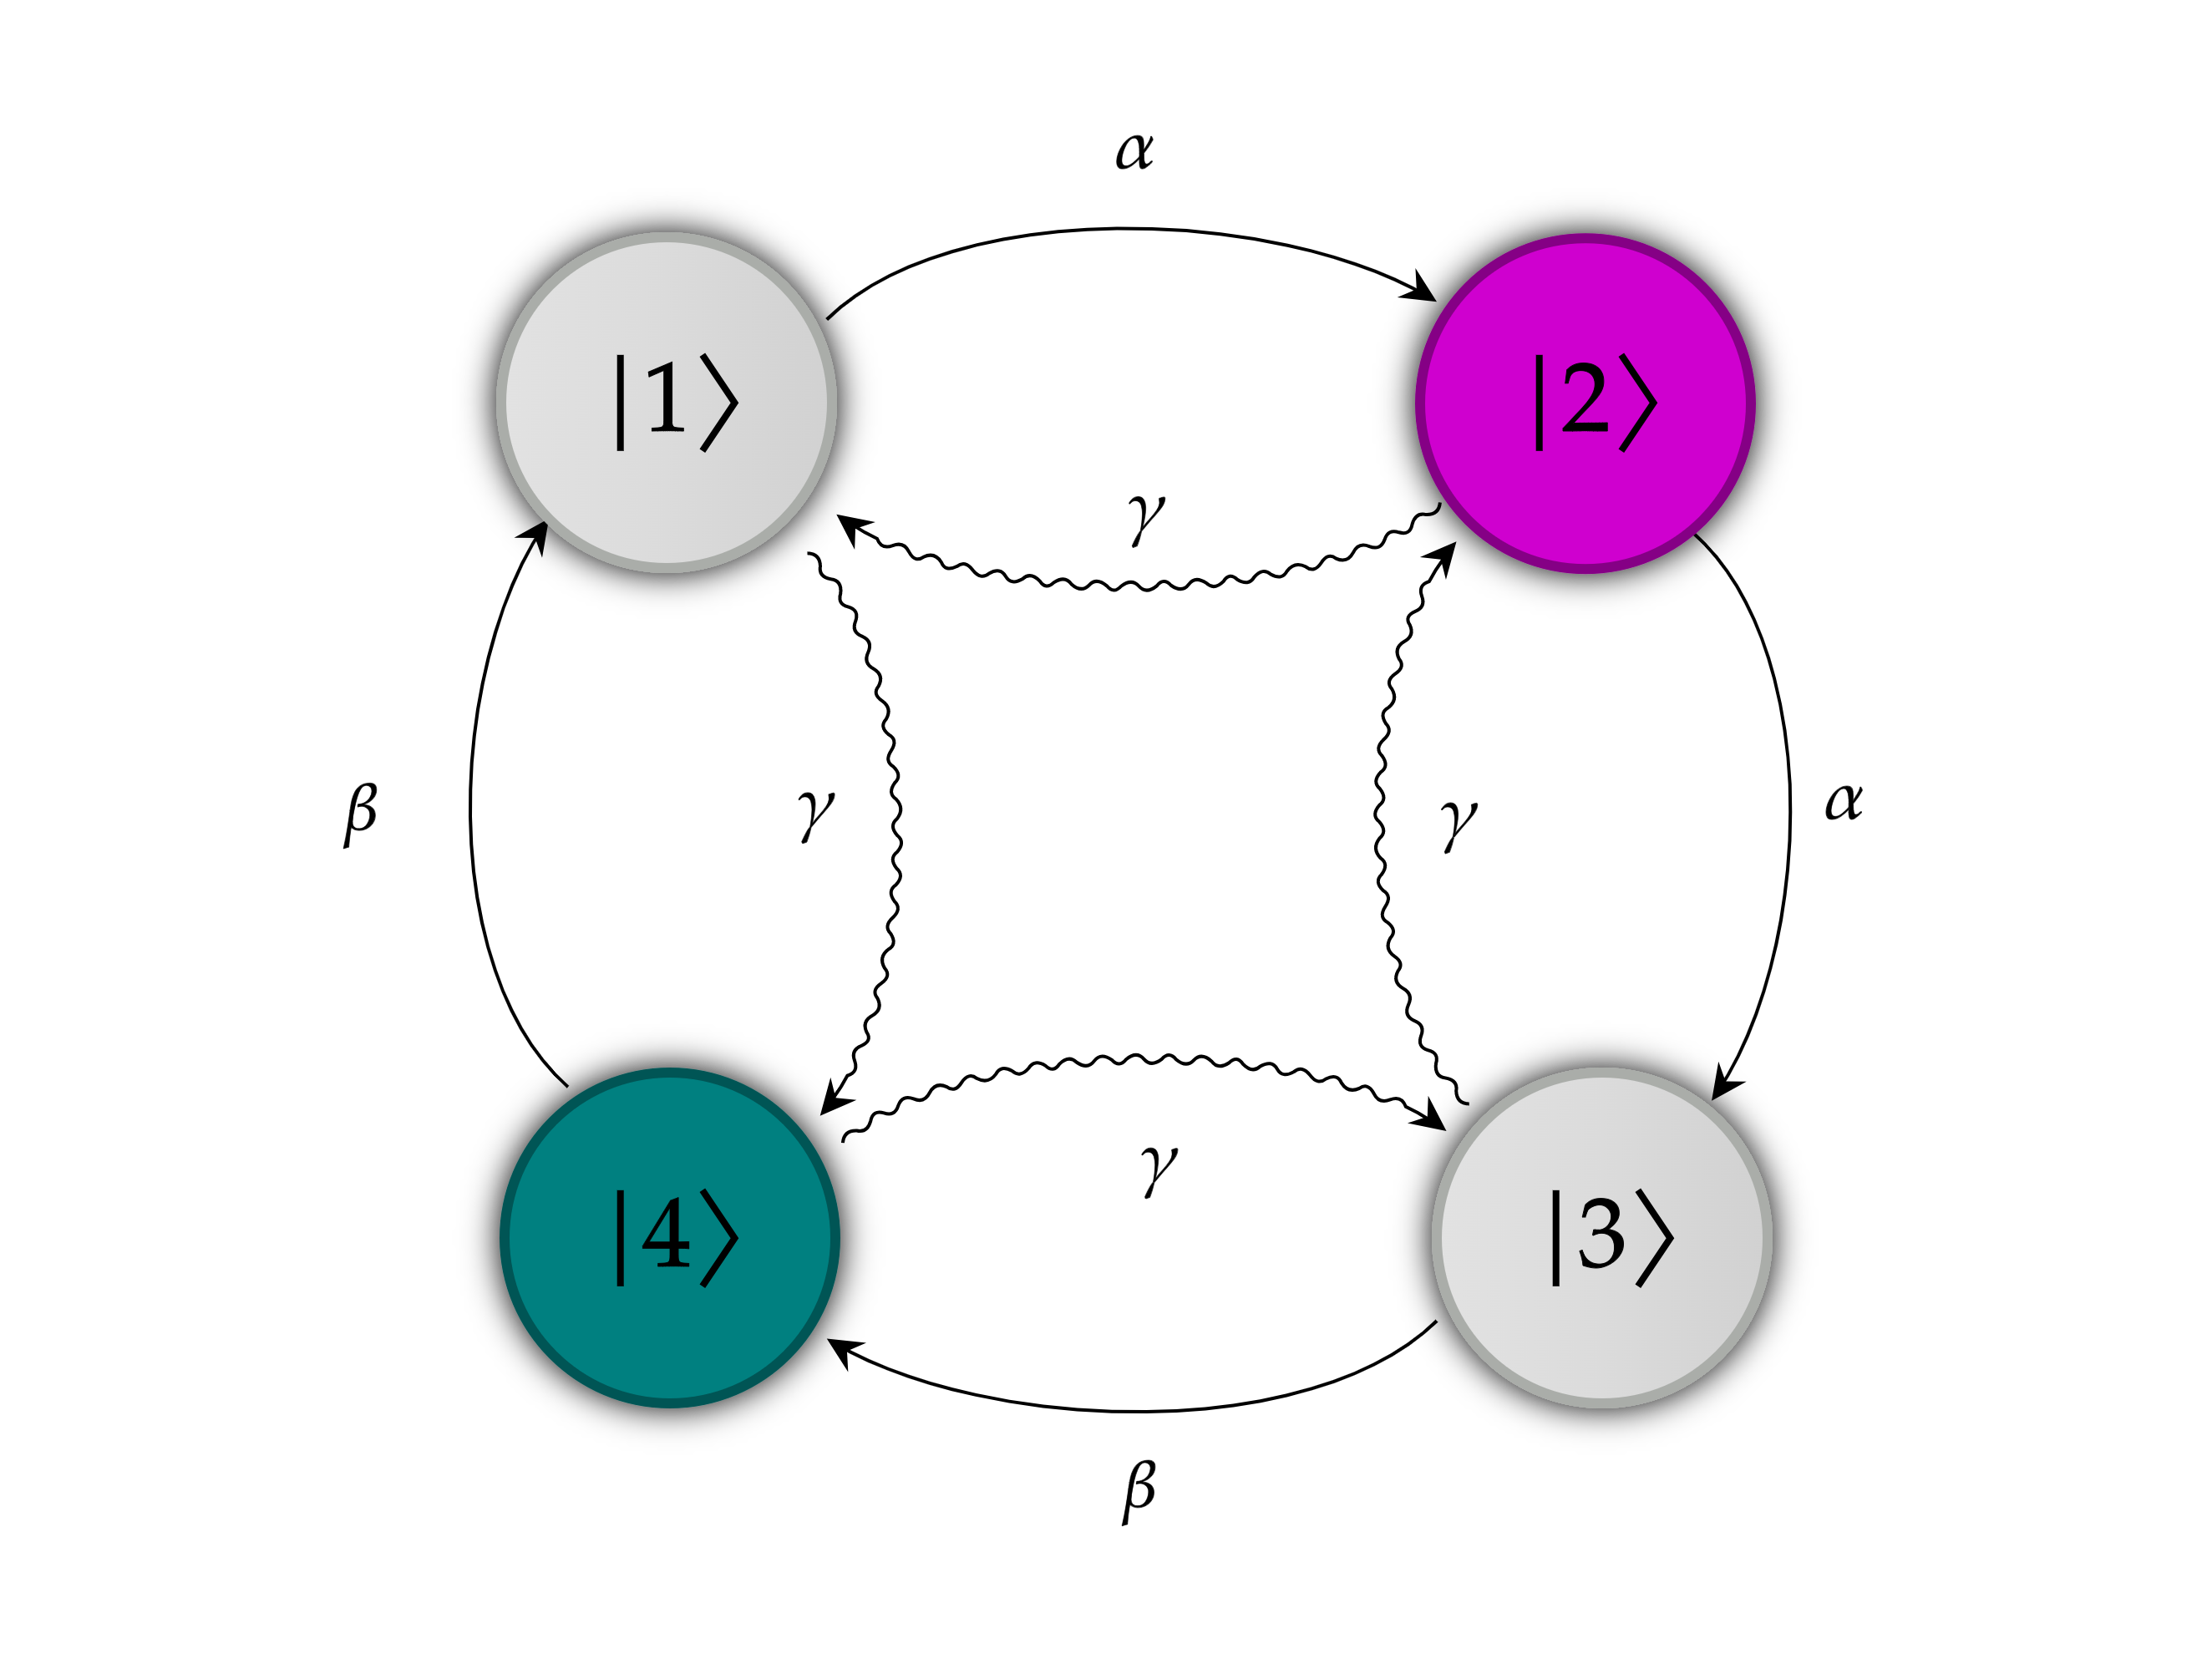
\includegraphics[width = \textwidth]{figures/waiting_room.png}
  \caption{Granular waiting room}
  \label{granular_fig}
\end{subfigure}
\begin{subfigure}[b]{0.49\textwidth}
  \centering
  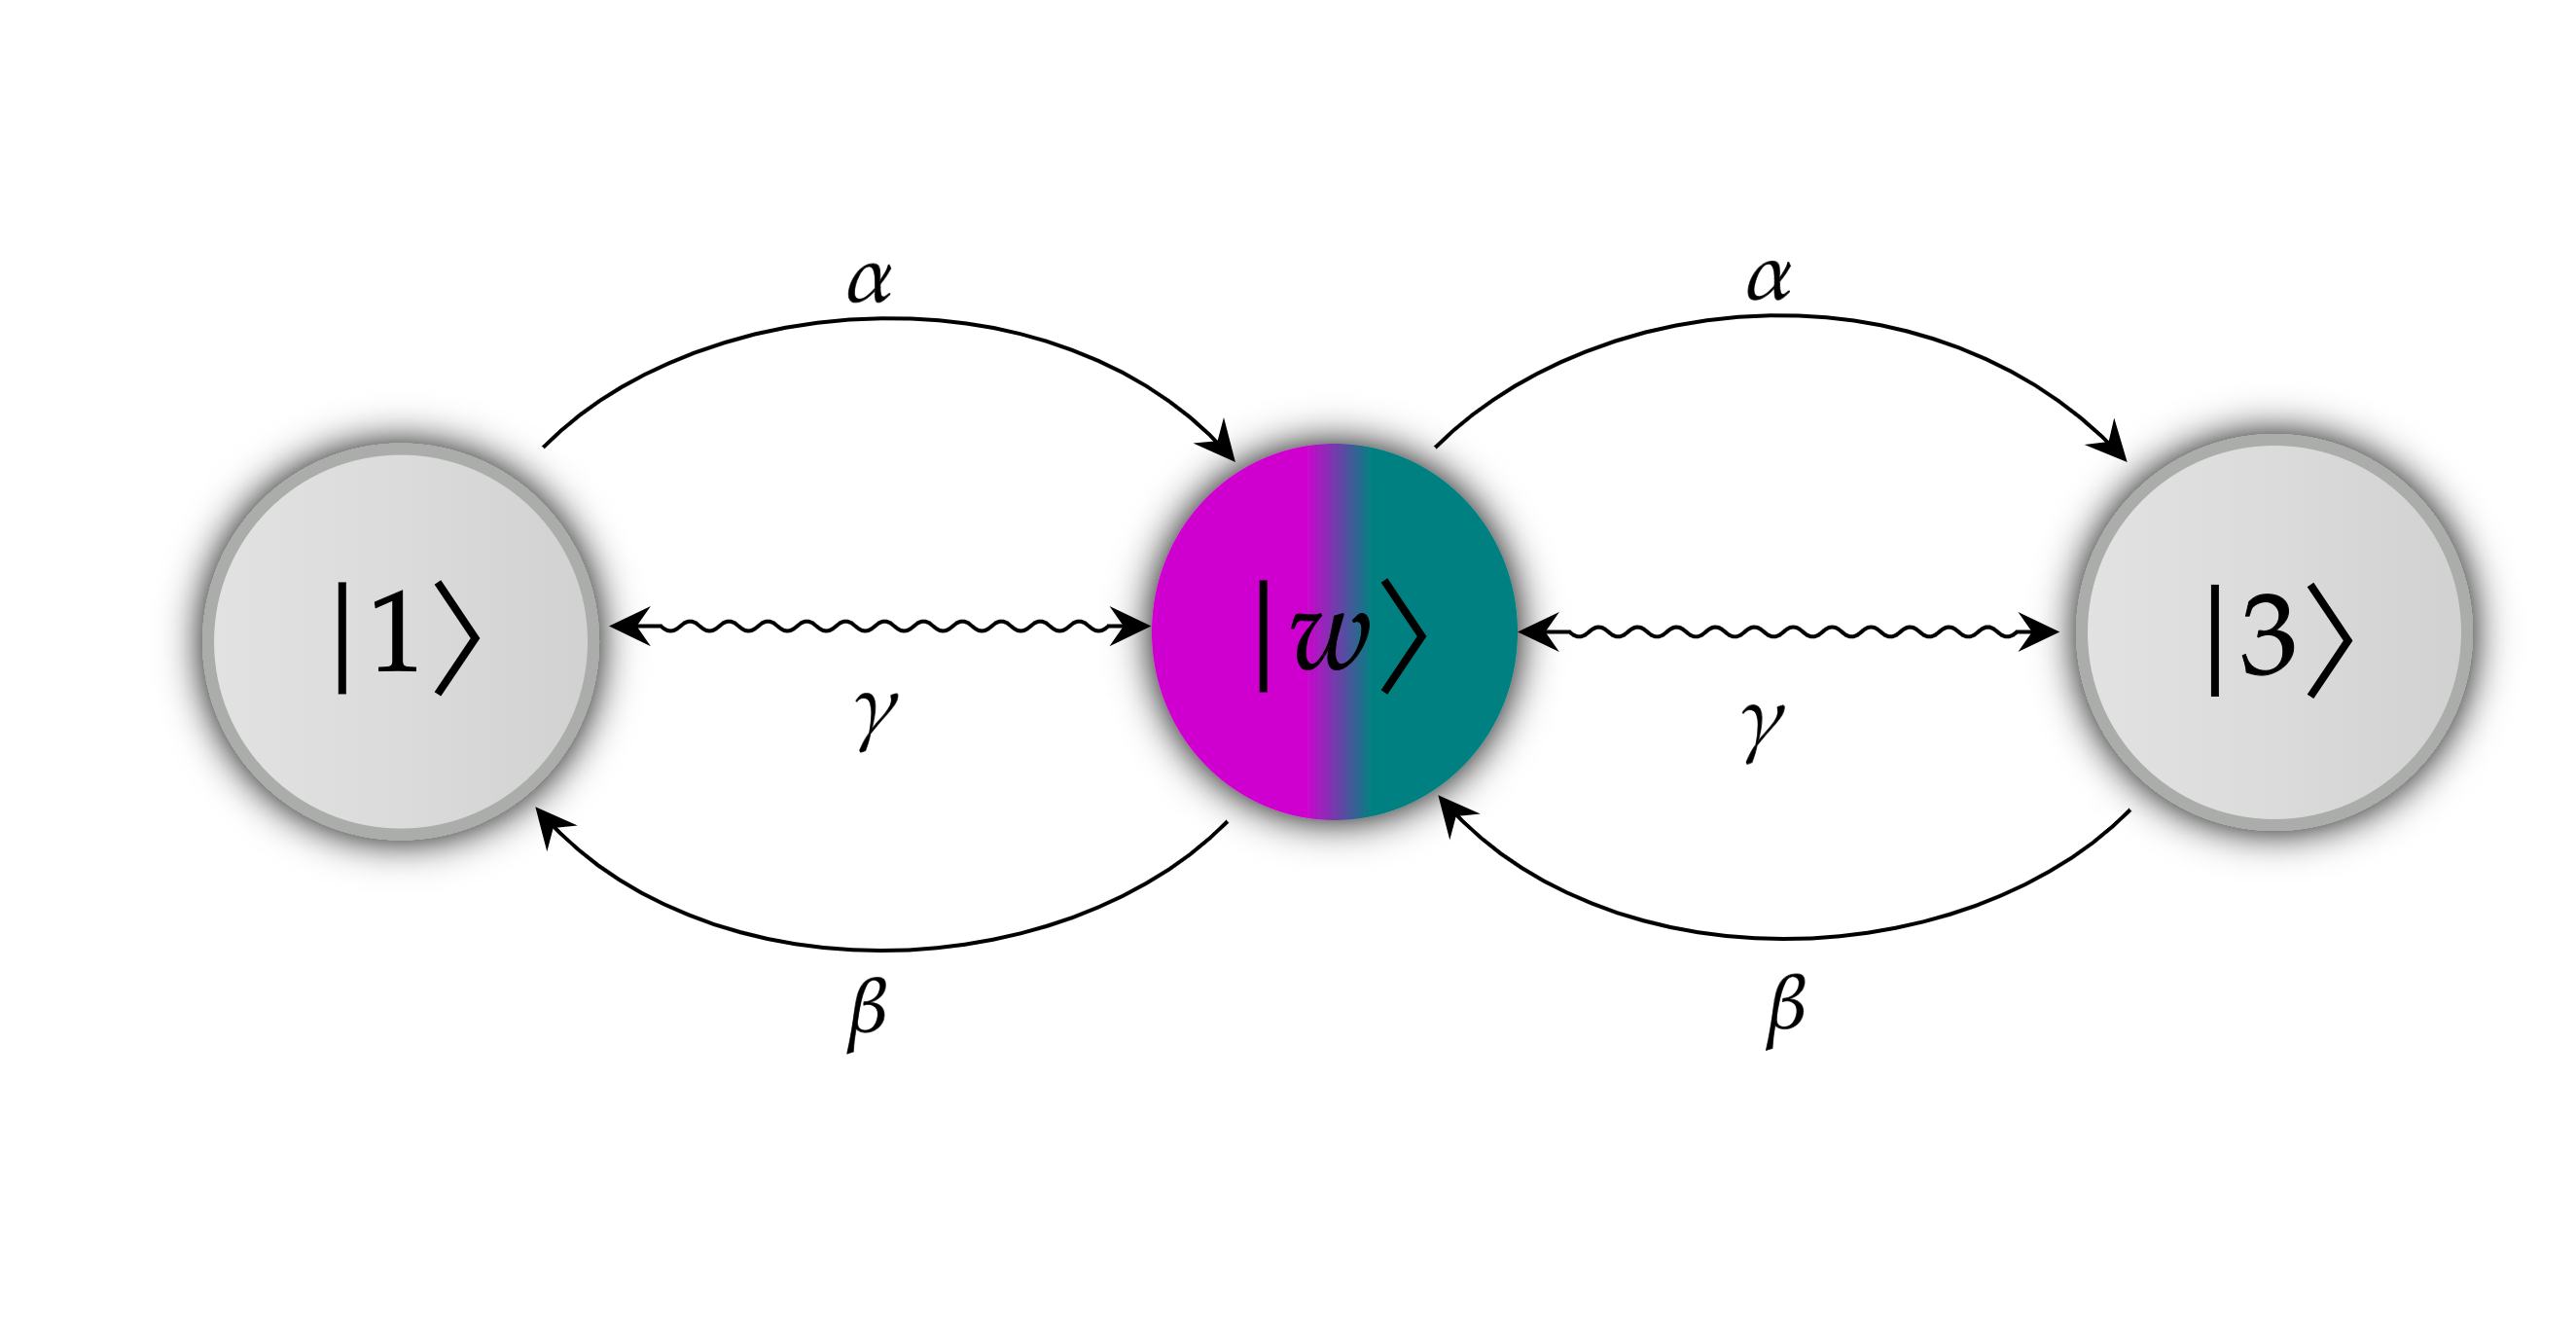
\includegraphics[width = \textwidth]{figures/wait_room_coarse.png}
  \caption{The waiting room}
  \label{coarse_grained_fig}
\end{subfigure}
\caption{\footnotesize Subfigure \ref{granular_fig} shows the granular Waiting Room (WR) system while \ref{coarse_grained_fig} shows the WR. Note that in the WR, there is no sense of cycle direction, i.e., to complete a cycle a particle must always traverse the state-space in the same order. This is in contrast to the granular WR where, starting from any state, a particle can cycle in the clockwise or anticlockwise directions. Depending on the values of the parameters $\alpha,\beta,$ and $\gamma$ this can lead to non-zero flux in the steady state of the granular WR. Meanwhile the WR cannot accommodate any net current in its steady state.}
\label{system_desc_fig}
\end{figure}

The system depicted in Figure \ref{granular_fig} is a Markov process with transition matrix

\begin{equation}
  W = W_{i \rightarrow j} = \begin{pmatrix}-\alpha - \gamma && \alpha && 0 && \gamma \\
\gamma && -\alpha - \gamma && \alpha && 0 \\
0 && \gamma && -\beta-\gamma && \beta \\
\beta && 0 && \gamma && -\beta - \gamma \end{pmatrix}.
\end{equation}

Henceforth we shall call this the granular `Waiting Room' (WR) system. As in Section \ref{two_state_path_prob}, it is possible to write down the density of paths around any given path by conditioning on the number of jumps made by a particle in the granular (WR) system. The added complication in this case is that the density will not only depend on the number of jumps, but also on the type of each jump (e.g. the density of paths making one jump of the type $\ket{1} \rightarrow \ket{2}$ is different to those making one jump of the type $\ket{1} \rightarrow \ket{4}$).

\begin{wrapfigure}{R}{0.4\textwidth}
    \centering
    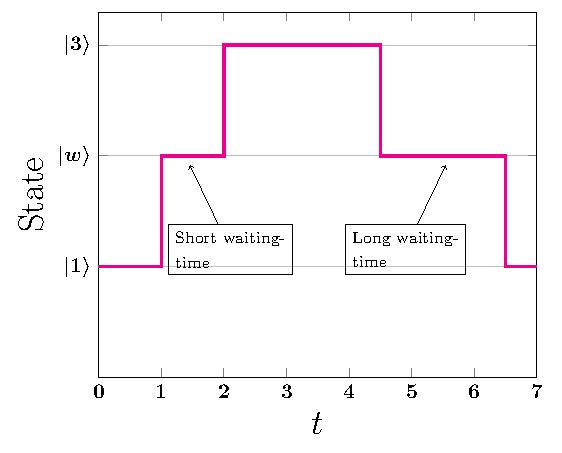
\includegraphics[width = 0.35\textwidth]{figures/waiting_room_sample_path.pdf}
    \caption{ \footnotesize A typical path for the WR system. For this path we assume $\alpha > \beta > \gamma$. The particle jumps from state $\ket{1}$ to $\ket{w}$ at $t = 1$ then to $\ket{3}$ at $t = 2$. It then climbs back down to $\ket{w}$ and eventually to $\ket{1}$. Since the system is much more likely to be in $\ket{2}$ if it has entered $\ket{w}$ from $\ket{1}$ (as it does at time $t = 1$), the expected waiting time in this case is much smaller than the case where the system enters $\ket{w}$ from $\ket{3}$ (as it does at $t = 4.5$), in which case it is most likely to have entered state $\ket{4}$ in the granular description. It is clear from this picture that the forward and reverse paths have different statistics.}
    \label{fig:coarse_grained_sample_path}
\end{wrapfigure}

From this granular WR system we obtain the WR system by collapsing the states $\ket{2}$ and $\ket{4}$ together as in Figure \ref{coarse_grained_fig}. The combination state obtained by this procedure we shall call $\ket{w}$. This coarse-grained system is no longer Markov since observed waiting times of the particle in $\ket{w}$ inform the inferred state of the system. It is also intuitively clear that the coarse-grained system has non-zero entropy production along its paths. See for example Figure \ref{fig:coarse_grained_sample_path} which shows a cartoon of a sample path. This cartoon makes evident the fact that the statistics of the forward and reverse paths are not equivalent. Our goal is to calculate the long-time expectation value for the Kullback-Leibler divergence of the coarse-grained paths. In doing so, we will assume that the system occupies its stationary state throughout. The most important implication of this assumption is that the time evolution of the measure of the process will no longer contribute to the entropy production as it did for the telegraph process in Section \ref{chapter:telegraph}. 

Each state in the granular system has an exponential waiting-time distribution $\psi_{\ket{i}}(t)$. This is distinct from the distribution of a transition $\ket{i} \rightarrow \ket{j}$ which we denote by $\psi_{ij}(t)$. The probability that a transition away from $\ket{i}$ is of the type $\ket{i} \rightarrow \ket{j}$ is then

\begin{equation}
    P_{ij} = \int_0^\infty \psi_{i j}(t)dt.
\end{equation}

The waiting time distribution conditioned on a given transition is then the normalised distribution $\psi_{ij}(t)/P_{ij}$. For example, using the methodology from Section II, we derive for state $\ket{1}$

\begin{align}
    \begin{split}
        \psi_{\ket{1}}(t) &= (\alpha + \gamma) e^{-(\alpha + \gamma)t},\\
        \psi_{12}(t) &= \alpha e^{-(\alpha + \gamma)t},\\
        \psi_{14}(t) &= \gamma e^{-(\alpha + \gamma)t},
    \end{split}
\end{align}

whereby $P_{12} = \frac{\alpha}{\alpha + \gamma}$, and $P_{14} = \frac{ \gamma}{ \alpha + \gamma}$ follow straightforwardly. Note that $\psi_{12}$ and $\psi_{14}$ are not normalised. The stationary distribution of the granular WR is given by 

\begin{align}\label{granular}
\begin{split}
\mu_1 &= \frac{1}{Z} \left(\alpha \alpha\beta^2 + \gamma(\beta^2 +\beta\gamma + \gamma^2) \right),\\
\mu_2 &= \frac{1}{Z}\left(\gamma^3 + \alpha(\beta^2 + \beta\gamma + \gamma^2)\right),\\ 
\mu_3 &= \frac{1}{Z}\left(\alpha\gamma^2 + \gamma^3 +\alpha^2(\beta+\gamma)\right),\\ 
\mu_4 &= \frac{1}{Z}\left(\alpha^2\beta +\alpha\beta\gamma+\gamma^2(\beta+\gamma)\right),\\
Z &= 2\alpha\beta(\alpha + \beta) +(\alpha+\beta)^2\gamma+2(\alpha+\beta)\gamma^2 +4\gamma^3.
\end{split}
\end{align}

The granular WR is a Markov chain, so we may calculate its steady-state entropy production rate according to \cite{schnakenberg1976network}

\begin{align}
\entpp_G = r\mathcal{A},
\end{align}

where $r$ is the \textit{clockwise} current of the system as seen in Figure \ref{granular_fig}, and 

\begin{align}
\mathcal{A} = \log\left (\frac{\alpha^2\beta^2}{\gamma^4}\right)
\end{align}

is the cycle affinity. Let $r_{ij} = r_{i \rightarrow j}$ be the current from $\ket{i}$ to $\ket{j}$. Then 
\begin{align}
r_{12} = \alpha \mu_1 - \gamma \mu_2 = \frac{1}{Z}(\alpha^2\beta^2-\gamma^2).
\end{align}
On the other hand, a simple application of Kirchoff's law yields, 
\begin{align}
r_{12} = r_{23} = r_{34} = r_{41},
\end{align}
hence $r = r_{12}/4$ and 
\begin{align}\label{granular-waiting-entropy-close}
\entpp^g = \frac{\alpha^2\beta^2-\gamma^4}{4Z}\log\left(\frac{\alpha^2\beta^2}{\gamma^4} \right).
\end{align}

We stress that in the WR, the state $\ket{w}$ does not indicate a particular combination state of $\ket{2}$ and $\ket{4}$, but any convex linear combination state $a\ket{2} + b\ket{4}$. The observer only has access to $\ket{w}$, but they may infer a probabilistic combination of $\ket{2}$ and $\ket{4}$ based on the system's history. In particular, if a state $\ket{\bar{w}} = a\ket{2} + b\ket{4}$ is inferred at $t = 0$, and the system has made no jumps in time $t$, then it occupies the combination state 

\begin{align}\label{waiting-room-timeevol}
\ket{\bar{w}(t)} = \frac{1}{a e^{-(\alpha + \gamma)t} + b e^{-(\beta + \gamma)t}}\left (a e^{-(\alpha + \gamma)t}\ket{2} + b e^{-(\beta + \gamma)t}  \ket{4}\right).
\end{align}

We may say that $\ket{w}$ is an \emph{observed} or observable state of the system, while $\ket{\bar{w}(t)}$ is an \emph{inferred} state.  

\subsection{Discrete Time Treatment}
\subsubsection{Path-Histories and Gluing Scheme}
\label{subsection:path-histories}

We will first treat this system in discrete time with time step $\tau$. Write $M = \mathds{1} + \tau W$ for the stochastic matrix of the discretised process. To avoid burdensome notation, we will write $(\ket{i}, m)$, for $i \in \{1, w, 3 \}$ and $m \in \bN \cup \{0\}$ to mean that the system was in state $\ket{i}$ for time $m\tau$. For any path $\omega$ beginning in $\ket{1}$ and ending in $\ket{3}$ the history of $\omega$ can be written

$$\{(\ket{1}, n_1), (\ket{w}, n_2), (\ket{3}, n_3), (\ket{w}, n_4), (\ket{1}, n_5), \ldots (\ket{3}, n_N)\}.$$

For example, if the path is given by $\omega = \ket{1}\xrightarrow{3}{} \ket{w} \xrightarrow{2}{} \ket{1} \xrightarrow{5}{} \ket{w} \xrightarrow{4}{} \ket{3}$ then we will have $n_1 = 3, n_2 =2, n_3 = n_4 = 0, n_5 = 5, n_6 = 4$.  Given a history in the form $\mathcal{P} = \{i_1, i_2, i_3, \ldots, i_N\}$ in the granular system, where the $i_k$ are states, we know that the probability of the path described by $\mathcal{P}$ is given by

$$\bP(\mathcal{P}) = \bra{i_1}M\ket{i_2}\bra{i_2}M\ket{i_3}\ldots\ket{i_{N-1}}\bra{i_{N-1}}M\ket{i_N}.$$

Let now $\bar{\mathcal{P}} = \{(\ket{i},2),(\ket{w},2),(\ket{j},2)\}$, $i,j \in \{1,3\}$ be a path in the coarse grained system. The particle jumping from $\ket{i}$ to $\ket{w}$ may have entered state $\ket{2}$ or $\ket{4}$, so the path probability for $\bar{\mathcal{P}}$ can be written

\begin{equation}
  \bP (\bar{\mathcal{P}}) = \bra{i}M\ket{i}\bra{i}M\bigg(\ket{2}\bra{2}+\ket{4}\bra{4}\bigg)M\ket{j}\bra{j}M\ket{j}
\end{equation}

To simplify the act of summing up over large subsets of paths, we would like to factorise the bracket on the RHS of the above to write

\begin{equation}\label{wrong_exper}
    \bra{i}M\ket{i}\bra{i}M\big(\ket{2}+\ket{4}\big)\big(\bra{2}+\bra{4})M\ket{j}\bra{j}M\ket{j}
\end{equation}

but note that (\ref{wrong_exper}) gives rise to invalid paths such as

$$\bra{i}M\ket{i}\bra{i}M\ket{2}\bra{4}M\ket{j}\bra{j}M\ket{j}. $$

This path is invalid because it ends the third time step in state $\ket{2}$ but begins the fourth time step in $\ket{4}$. This is not allowed since no time elapses between the end of one time step and the beginning of the next. To resolve this issue we shall use a `gluing' scheme. Denoting by $\bar{z}$ the complex conjugate of $z$, We write

\begin{equation}
  \bP (\bar{\mathcal{P}}) = \frac{1}{2\pi}\int_{\abs{z} \leq 1}d^2z\bra{i}M\ket{i}\bra{i}M\bigg(z\ket{2} + \ket{4}\bar{z}\bigg)\bigg(\bra{2}\bar{z}+ \bra{4}z \bigg)M\ket{j}\bra{j}M\ket{j},
\end{equation}

making use of the fact that

\begin{equation}
  \int_{\abs{z}\leq 1} d^2z \:z^2 = 0, \quad \quad \int_{\abs{z}\leq 1}d^2z \:\abs{z}^2 = 2\pi.
\end{equation}

If we now define

\begin{align}
  J_n \coloneqq \frac{1}{(2\pi)^n} \int_{\abs{z_1} \leq 1}d^2z_1\int_{\abs{z_1} \leq 1}d^2z_2\ldots \int_{\abs{z_n} \leq 1}d^2z_n \big(z_1\ket{2} + \ket{4}\bar{z}_1\big)&\big(\bra{2}\bar{z}_1+ \bra{4}z_1 \big)M\ldots \nonumber \\  & M\big(z_n\ket{2} + \ket{4}\bar{z}_n\big)\big(\bra{2}\bar{z}_n+ \bra{4}z_n \big),
\end{align}

then the probability of any path can be easily written in terms of the $J_n$'s. Considering again the path $\omega$ with history $\{(\ket{1}, n_1), (\ket{w}, n_2), (\ket{3}, n_3), (\ket{w}, n_4), (\ket{1}, n_5), \ldots (\ket{3}, n_N)\}$, we can now write

\begin{align}\label{simple_glued_path_prob}
  \bP(\omega) = \bra{1}M\ket{1}^{n_1}\bra{1}MJ_{n_2}M\ket{3}\bra{3}M\ket{3}^{n_3}\ldots \bra{1}MJ_{n_{N-1}}M\ket{3}\bra{3}M\ket{3}^{n_N}
\end{align}

This is still not the form we will use to find the expectation value of the Kullback-Leibler divergence, however the above expression does make clear a very important qualitative feature of the entropy production in the WR system. Studying the RHS of Equation (\ref{simple_glued_path_prob}), we note that the only scalar terms which are not stable under time reversal are those of the form $\bra{1}MJ_{n_i}M\ket{3}$ and $\bra{3}MJ_{n_i}M\ket{1}$. Hence, writing $\omega^\ast$ for the time reversed path corresponding to $\omega$, we have

\begin{equation}
  \frac{\bP(\omega)}{\bP(\omega^\ast)} = \frac{\bra{1}MJ_{n_2}M\ket{3}}{\bra{3}MJ_{n_2}M\ket{1}}\frac{\bra{1}MJ_{n_4}M\ket{3}}{\bra{3}MJ_{n_4}M\ket{1}}\ldots\frac{\bra{1}MJ_{n_{N-1}}M\ket{3}}{\bra{3}MJ_{n_{N-1}}M\ket{1}}.
\end{equation}

Taking the logarithm this is

\begin{equation}\label{where_prod_entropy}
  \log\left(\frac{\bP(\omega)}{\bP(\omega^\ast)} \right) = \log \left(\frac{\bra{1}MJ_{n_2}M\ket{3}}{\bra{3}MJ_{n_2}M\ket{1}} \right) + \log \left(\frac{\bra{3}MJ_{n_4}M\ket{1}}{\bra{1}MJ_{n_4}M\ket{3}} \right) + \ldots
  \log \left ( \frac{\bra{1}MJ_{n_{N-1}}M\ket{3}}{\bra{3}MJ_{n_{N-1}}M\ket{1}}\right).
\end{equation}

Equation \ref{where_prod_entropy} says that the entropy produced along $\omega$ is precisely the entropy produced along the sections of $\omega$ where the system travels from $\ket{1}$ to $\ket{3}$ (or vice versa) through $\ket{w}$. In particular, no terms of the form $\bra{1}MJ_{n_i}M\ket{1}$ or $\bra{3}MJ_{n_i}M\ket{3}$ appear in the logarithm, which is to say that if an excursion away from state $\ket{1}$ (respectively $\ket{3}$) ends before visiting state $\ket{3}$ (respectively $\ket{1}$) then \textit{it will not contribute to the entropy production of the path.}

Another important implication is that the expectation $ \bE\left[ \log\left(\frac{\bP(\omega)}{\bP(\omega^\ast)}\right)\right]$ breaks down into (relatively) simple sums. Letting $\Omega$ be the space of all paths for the coarse-grained system, We have

\begin{align}\label{broken_expec}
    \bE\left[ \log\left(\frac{\bP(\omega)}{\bP(\omega^\ast)}\right)\right] &= \sum_{\Omega} \bP(\omega)\log\left(\frac{\bP(\omega)}{\bP(\omega^\ast)}\right) \nonumber\\
    &= \sum_{\Omega} \bP(\omega)\log\left(\frac{\bra{1}MJ_{n_4}M\ket{3}}{\bra{3}MJ_{n_4}M\ket{1}}\right) +  \sum_{\Omega} \bP(\omega)\log\left(\frac{\bra{1}MJ_{n_{2}}M\ket{3}}{\bra{3}MJ_{n_{2}}M\ket{1}}\right) + \ldots \nonumber \\ &\qquad + \sum_{\Omega} \bP(\omega)\log\left(\frac{\bra{1}MJ_{n_{N-1}}M\ket{3}}{\bra{3}MJ_{n_{N-1}}M\ket{1}}\right).
\end{align}

This decomposition motivates the splitting of paths into sections that travel from $\ket{1}$ to $\ket{3}$ and vice-versa. Such sections we shall call half cycles.

\subsubsection{Half Cycles}
\label{subsection:half-cycles}

Let us define the stopping times

\begin{align}
    \begin{split}
  T_3 &= \inf\{n > 0: \ket{x_n} = \ket{3} \}, \\
  T_1 &= \inf\{ n > 0: \ket{x_n} = \ket{1} \}.
    \end{split}
\end{align}

Certainly, $\bE(T_3 \; | \; \ket{x_0} = \ket{1}) < \infty$.\footnote{Since the underlying granular WR is a finite Markov chain, i.e., it is recurrent.} So, we may ask \textit{what is the expected entropy production, $\mathcal{S}_{1 \rightarrow 3}$, up to time $T_3$, beginning from $\ket{1}$?}

The probability for any path from $t = 0$ to $T_3$ can be written

\begin{equation}\label{half-cycle-prob}
\bP(\omega) = \bra{x_0 = 1}m_1\ket{1}\bra{1}MJ_{n_1}M\ket{1}\bra{1}m_2\ket{1}\ldots\bra{1}m_N\ket{1}\bra{1}MJ_{n_N}M\ket{3}.
\end{equation}

Here the $m_i$ and the $n_i$ are the duration, in time steps, of the $i$-th visit to $\ket{1}$ and $\ket{w}$ respectively. $\bra{1}m\ket{1}$ denotes the path segment

\begin{equation}
    \bra{1}m\ket{1} = \underbrace{\bra{1}M\ket{1}\bra{1}M\ldots M\ket{1}}_{\text{$m$ steps}}.
\end{equation}

Now, at time $T_1$ the an observer of the WR has access to the same description as an observer of the granular WR, hence the process can be thought of as restrating at time $T_1$.\footnote{See Section \ref{chapter:classification} for a discussion} Likewise at $T_3$. Therefore the times $m_i > 0$ and $n_i > 0$ are independent. Eqn. (\ref{half-cycle-prob}) is the probability of a path which takes $N$ excursion from $\ket{1}$ before visiting $\ket{3}$. Let us define the state

\begin{equation}\label{w1_comb_state}
    \ket{w_1} = \frac{\alpha}{\alpha + \gamma} \ket{2} +  \frac{\gamma}{\alpha + \gamma} \ket{4}.
\end{equation}
$\ket{w_1}$ is the \emph{inferred} state of the system immediately after a jump $\ket{1} \rightarrow \ket{w}$. This is as opposed to $\ket{w}$ which is the \emph{observed} state. Beginning from $\ket{w_1}$ the probability that the next jump is to $\ket{3}$ is given by

\begin{align}
\begin{split}
P(\ket{w_1}\rightarrow \ket{3}) &= \frac{\alpha}{\alpha + \gamma} P(\ket{2} \rightarrow \ket{3}) + \frac{\gamma}{\alpha + \gamma} P(\ket{4} \rightarrow \ket{2}) \\
&= \frac{\alpha^2}{(\alpha + \gamma)^2} +  \frac{\gamma^2}{(\alpha + \gamma)(\beta +\gamma)} \eqqcolon p
\end{split}
\end{align}


Let $\mathcal{N}$ be the random variable indicating the number of excursions made from $\ket{1}$ before $\ket{3}$ is reached. Then $\mathcal{N}$ is a geometric r.v. such that

\begin{align}
\begin{split}
P\left(\mathcal{N} = N\right) &= p(1-p)^{N-1} \\
\bE \mathcal{N} &= 1/p.
\end{split}
\end{align}

Observe that

\begin{align}
\sum_{n_i,m_i}^\infty \bra{1}m_1\ket{1}\bra{1}MJ_{n_1}M\ket{1}\ldots\bra{1}m_N\ket{1}\bra{1}MJ_{n_N}M\ket{3} = P(\mathcal{N} = N).
\end{align}

Then we will have for the entropy production up to time $T_3$,

\begin{align}\label{half-cycle-EP}
\small
\begin{split}
    \mathcal{S}_{1 \rightarrow 3} &= \sum_{\Omega}\bP(\omega)\log\left ( \frac{\bra{1}MJ_{n_N}M\ket{3}}{\bra{3}MJ_{n_N}M\ket{1}}\right) \\
    &= \sum_{N=1}^\infty \sum_{m_i,n_i}^\infty \bra{ 1}m_1\ket{1}\bra{1}MJ_{n_1}M\ket{1}\ldots\bra{1}m_N\ket{1}\bra{1}MJ_{n_N}M\ket{3} \log\left ( \frac{\bra{1}MJ_{n_N}M\ket{3}}{\bra{3}MJ_{n_N}M\ket{1}}\right) \\
    &= \left[\sum_{N=1}^\infty \sum_{m_i, n_i}\bra{1}m_i\ket{1}\ldots\bra{1}m_{N-1}\ket{1}\bra{1}MJ_{n_{N-1}}M\ket{1} \right] \sum_{m_N,n_N}^\infty \bra{1}m_N\ket{1}\bra{1}MJ_{n_N}M\ket{3}\log\left( \frac{\bra{1}MJ_{n_N}M\ket{3}}{\bra{3}MJ_{n_N}M\ket{1}}\right) \\
    &= \left(\sum_{N=1}P(\mathcal{N} \geq N)\right)\sum_{m,n}^\infty \bra{1}m\ket{1}\bra{1}MJ_{n}M\ket{3}\log\left( \frac{\bra{1}MJ_{n}M\ket{3}}{\bra{3}MJ_{n}M\ket{1}}\right) \\
    &= \bE \mathcal{N} \sum_{m,n}^\infty \bra{1}m\ket{1}\bra{1}MJ_{n}M\ket{3}\log\left( \frac{\bra{1}MJ_{n}M\ket{3}}{\bra{3}MJ_{n}M\ket{1}}\right) \\
    &= \frac{1}{p} \sum_{m,n}^\infty \bra{1}m\ket{1}\bra{1}MJ_{n}M\ket{3}\log\left( \frac{\bra{1}MJ_{n}M\ket{3}}{\bra{3}MJ_{n}M\ket{1}}\right).
\end{split}
\end{align}

Now, using the same methodology as in Section II, we obtain

\begin{align}
\bra{1}m\ket{1}\bra{1}MJ_{n}M\ket{3} \xrightarrow{\tau \rightarrow \rmd t} \rmd t_1 \rmd t_2 \alpha^2 e^{-(\alpha + \gamma)t_1}\left(e^{-(\alpha + \gamma)(t_2-t_1)} + \frac{\gamma^2}{\alpha^2}e^{-(\beta+\gamma)(t_2-t_1)}\right).
\end{align}

Moreover, using the definition of $J_n$ we have

% \begin{align}
% \bra{1}MJ_{n}M\ket{3} = \alpha \tau \bra{2}MJ_{n-1}M\ket{3} + \gamma \tau \bra{4}MJ_{n-1}M\ket{3},
% \end{align}

% and similar for $\bra{3}MJ_{n}M\ket{1}$ such that in the continuous-time limit (\ref{half-cycle-EP}) becomes

We must proceed with caution in evaluating the logorithm $\log\left( \frac{\bra{1}MJ_{n}M\ket{3}}{\bra{3}MJ_{n}M\ket{1}}\right)$ in the continuous time limit. Naively, one may think that in the continuous time limit $\bra{1}MJ_nM\ket{3}$ becomes the density of paths making a transition $\ket{1} \rightarrow \ket{w}$ at time $t = 0$ and proceeding to visit $\ket{3}$ during this excursion. These are precisely the paths initialised at $\ket{w_1}$ which have $T_3 < T_1$. The density of such paths is 

\begin{align}\label{naive-density}
\bP(\ket{w_1}\xrightarrow{t} \ket{3}) = \left(\frac{\alpha^2}{\alpha + \gamma}e^{-(\alpha +\gamma)t} + \frac{\gamma^2}{\alpha+ \gamma} e^{-(\beta + \gamma)t}\right)\rmd t.
\end{align}

Notice that (\ref{naive-density}) is not normalised. However, in writing 

\begin{align} 
\log\frac{\bP(\omega)}{\bP(\omega^\ast)} = \log\left( \frac{\bra{1}MJ_{n_N}M\ket{3}}{\bra{3}MJ_{n_N}M\ket{1}}\right)
\end{align}

we have implicitly assumed that the forward path visits $\ket{3}$ for the first time on exactly the $N$-th excursion, i.e. the particle \textit{must} visit $\ket{3}$ during this excursion. Hence the density we seek is in fact 

\begin{align}
\bra{1}MJ_{n_N}M\ket{3} \xrightarrow{t}\bP \left [\ket{w_1} \xrightarrow[]{t}\ket{3} \; \bigg \lvert \; T_3 < T_1\right] = \frac{1}{p}\left(\frac{\alpha^2}{\alpha + \gamma}e^{-(\alpha +\gamma)t} + \frac{\gamma^2}{\alpha+ \gamma} e^{-(\beta + \gamma)t}\right)\rmd t,
\end{align}

which is a normalised density. Similarly, and for the same reasons, we have the limit 

\begin{align}
\bra{3}MJ_{n_N}M\ket{1} \xrightarrow{t}\bP \left [\ket{w_3}\xrightarrow[]{t}\ket{1} \; \bigg \lvert \; T_1 < T_3\right] =\frac{1}{p^\ast}\left(\frac{\beta^2}{\beta + \gamma}e^{-(\beta +\gamma)t} + \frac{\gamma^2}{\beta+ \gamma} e^{-(\alpha + \gamma)t}\right)\rmd t,
\end{align}

where

\begin{equation}
p^\ast = \frac{\beta^2}{(\beta + \gamma)^2}+ \frac{\gamma^2}{(\beta+\gamma)(\alpha + \gamma)}
\end{equation}

is the probability that a particular excursion from $\ket{3}$ visits $\ket{1}$ before returning to $\ket{3}$. So, in the continuous time limit 
\begin{align}\label{1to3_EP}
\begin{split}
\mathcal{S}_{1\rightarrow 3} &= \frac{1}{p}\int_0^\infty \rmd t_2 \int_0^{t_2} \rmd t_1 \alpha^2 e^{-(\alpha + \gamma)t_1}\left(e^{-(\alpha + \gamma)(t_2-t_1)} + \frac{\gamma^2}{\alpha^2}e^{-(\beta+\gamma)(t_2-t_1)}\right)\\
&\quad \quad \quad \log\left(\frac{p^\ast\alpha^2(\beta + \gamma)}{p\beta^2(\alpha + \gamma)}\frac{e^{-(\alpha + \gamma)(t_2-t1)}+ \gamma^2/\alpha^2e^{-(\beta +\gamma)(t_2-t_1)}}{e^{-(\beta + \gamma)(t_2-t_1)} + \gamma^2/\beta^2 e^{-(\alpha + \gamma)(t_2-t_1)}} \right)\\ 
& = \frac{1}{p}\frac{\alpha^2}{\alpha + \gamma} \int_0^\infty \rmd s \left(e^{-(\alpha + \gamma)s} + \frac{\gamma^2}{\alpha^2}e^{-(\beta+\gamma)s}\right)\log\left(\frac{p^\ast\alpha^2(\beta + \gamma)}{p\beta^2(\alpha + \gamma)}\frac{e^{-(\alpha + \gamma)s}+ \gamma^2/\alpha^2e^{-(\beta +\gamma)s}}{e^{-(\beta + \gamma)s} + \gamma^2/\beta^2 e^{-(\alpha + \gamma)s}} \right)
\end{split}
\end{align}

By symmetry, $\mathcal{S}_{3\rightarrow 1}$ is given by the integral

\begin{align}\label{3to1_EP}
\small
\begin{split}
\mathcal{S}_{3\rightarrow 1} = \frac{1}{p^\ast}\frac{\beta^2}{\beta + \gamma} \int_0^\infty \rmd s \left(e^{-(\beta + \gamma)s} + \frac{\gamma^2}{\beta^2}e^{-(\alpha+\gamma)s}\right)\log\left(\frac{p\beta^2(\alpha + \gamma)}{p^\ast\alpha^2(\beta + \gamma)}\frac{e^{-(\beta + \gamma)s}+ \gamma^2/\beta^2e^{-(\alpha +\gamma)s}}{e^{-(\alpha + \gamma)s} + \gamma^2/\alpha^2 e^{-(\beta + \gamma)s}} \right).
\end{split}
\end{align}

The entropy production rate of the WR is given by

\begin{align}
    \entpp^w = \frac{S_{1\rightarrow 3} + S_{3 \rightarrow 1}}{\bE_1T_3 + \bE_3T_1}.
\end{align}

The expectation $\bE_1T_3$ is the expectation value of $T_3$ given the particle is initialised in $\ket{1}$. This is the product of the expected number of excursions required to reach $\ket{3}$, equal to $1/p$, and the expected time taken for each excursion (including the time spent in $\ket{1}$). So,

\begin{align}
\begin{split} 
\bE_1T_3 &= \frac{1}{p} \bigg( \bE(\text{time spent in $\ket{1}$ during a visit}) + \bE (\text{time spent in $\ket{w_1}$ during a visit})\bigg)\\
&= \frac{1}{p}\left(\frac{1}{\alpha + \gamma} + \left (\frac{\alpha}{(\alpha +\gamma)^2} + \frac{\gamma}{(\alpha + \gamma)(\beta + \gamma)} \right)\right),
\end{split}
\end{align}

and similarly,

\begin{align}
\bE_3T_1 &= \frac{1}{p^\ast}\left(\frac{1}{\beta + \gamma} + \frac{\beta}{(\beta +\gamma)^2} + \frac{\gamma}{(\beta + \gamma)(\alpha + \gamma)} \right).
\end{align}

\subsection{Discussion}

\subsubsection{Entropy Production Results}

Figure \ref{fig:CG_waiting_room_entropy_prod} shows the entropy production rate of the WR process plotted against $\gamma/\beta$ for several values $\alpha/\beta$. The most salient features are the \text{finite} maximum of entropy production at $\gamma = 0$, the asymptotic approach to zero in the limit of large $\gamma$, and the intermediate dip which gives rise to zero entropy production at $\gamma/\beta = \sqrt{\alpha/\beta}$ . 

Since the case $\gamma = 0$ provides the most asymmetric cycle rates in the waiting room, it is unsurprising that the WR also has its maximum of entropy production at this point. In the granular system, however, setting $\gamma = 0$ results in infinite entropy production, since 'backwards' cycles (i.e. counterclockwise in Figure \ref{granular_fig}) are not possible in this case. Meanwhile the coarse grained system has a finite maximum of entropy production. This is because the particle must travel through $\ket{w}$ on its way during any half-cycle, regardless of the value of $\gamma$. Hence it is not possible to deterministically discern forward trajectories from reverse trajectories. This is in line with the general result \cite{maes2003time,}

\begin{align}\label{coarse-grained-inequality}
\entpp \geq \entpp_C,
\end{align}

where $\entpp$ is the entropy production of any system and $\entpp_C$ is the entropy production rate with some degrees of freedom hidden from the observer. 

As $\gamma$ grows large it masks the asymmetry in the waiting-time distributions of $\ket{w_1}$ and $\ket{w_2}$ , hence $\entpp^w$ approaches zero. How quickly the WR entropy production disappears is inversely related to  $\alpha/\beta$. Here again the granular WR and WR exhibit qualitatively different behaviours. For the granular WR, the current and cycle affinity approaches infinity as $\gamma$ goes to infinity, hence $\entpp^g$ diverges in this limit also. 

The entropy production of the WR is entirely due to asymmetric waiting-time distributions for $\ket{w_1}$ and $\ket{w_3}$ (see Subsection \ref{subsection:mechanism-wating-room}).  Supposing the WR observed in state $\ket{w_1(t)}$ or $\ket{w_2(t)}$ (given by Equation (\ref{w-evolutions})), the probability that the underlying granular WR occupies $\ket{2}$ is

\begin{align}
\bP\bigg( \ket{x(t)} = \ket{2} \: \bigg\lvert \: \ket{w_1(t)}\bigg) =& \frac{\alpha e^{-(\alpha + \gamma)t} }{\alpha e^{-(\alpha + \gamma)t}+ \gamma e^{-(\beta + \gamma)t}} \\ 
\bP\bigg( \ket{x(t)} = \ket{2} \: \bigg\lvert \: \ket{w_3(t)}\bigg) =& \frac{\gamma e^{-(\alpha + \gamma)t}}{\beta e^{-(\beta + \gamma)t} + \gamma e^{-(\alpha +\gamma)t}},
\end{align}

The statistics of the forward and reverse paths will be equal whenever the time-evolutions of these probabilities are indistinguishable. Let $\alpha = k\beta$. We have the ratio of probabilities 

\begin{align}\label{time-evolution-ratio}
\begin{split} 
\frac{\bP_{\ket{w_1}}(\ket{2})}{\bP_{\ket{w_3}}(\ket{2})} &= \left(\frac{k\beta e^{-(k\beta + \gamma)t} }{k\beta e^{-(\alpha + \gamma)t}+ \gamma e^{-(\beta + \gamma)t}}\right)\left(\frac{\gamma e^{-(k\beta + \gamma)t}}{\beta e^{-(\beta + \gamma)t} + \gamma e^{-(k\beta +\gamma)t}}\right)^{-1} \\
&= \frac{1}{k}\frac{\frac{\gamma}{\beta} \left(k + \frac{\gamma}{\beta} e^{-((1-k)\beta +\gamma)t}\right)}{e^{-((1-k)\beta +\gamma)t} + \frac{\gamma}{\beta}}.
\end{split}
\end{align}

For the time-evolutions to be indistinguishable, this ratio must equal unity. From (\ref{time-evolution-ratio}), we see that this condition is satisfied only when $\gamma/\beta = \sqrt{k}$. This explains the zero of entropy production at $\sqrt{\alpha/\beta}$ seen in Figure \ref{fig:CG_waiting_room_entropy_prod}. Indeed, since detailed balanced is satisfied in the granular WR  when $\gamma/\beta = \sqrt{\alpha/\beta}$, i.e. that process produces no entropy, Inequality (\ref{coarse-grained-inequality}) demands that the WR also produces no entropy in this case.

\begin{figure}
\centering
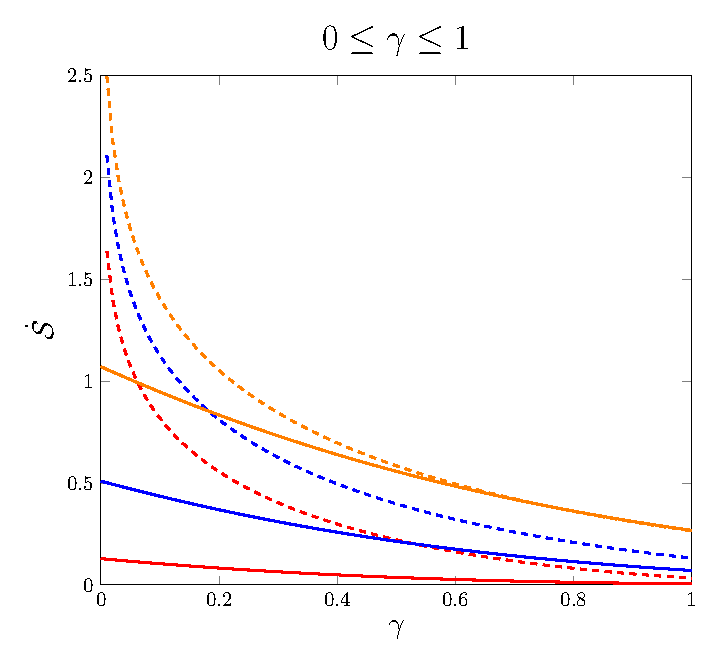
\includegraphics[width=0.32\textwidth]{figures/waiting_room_ent1.pdf}
%
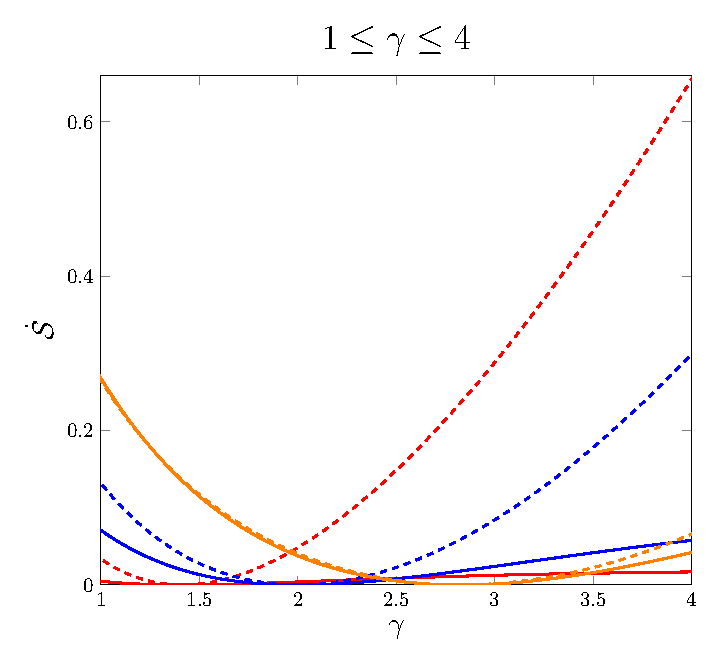
\includegraphics[width=0.32\textwidth]{figures/waiting_room_ent2.pdf}
%
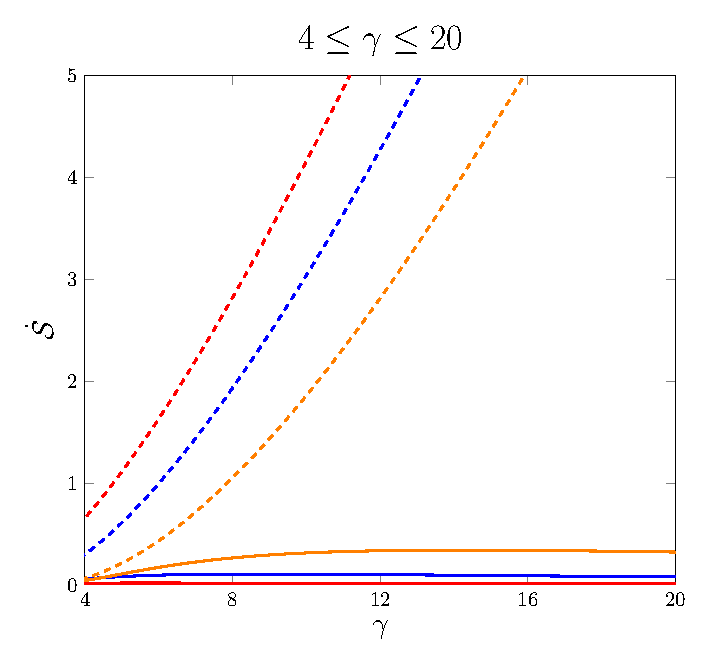
\includegraphics[width=0.32\textwidth]{figures/waiting_room_ent3.pdf}
%
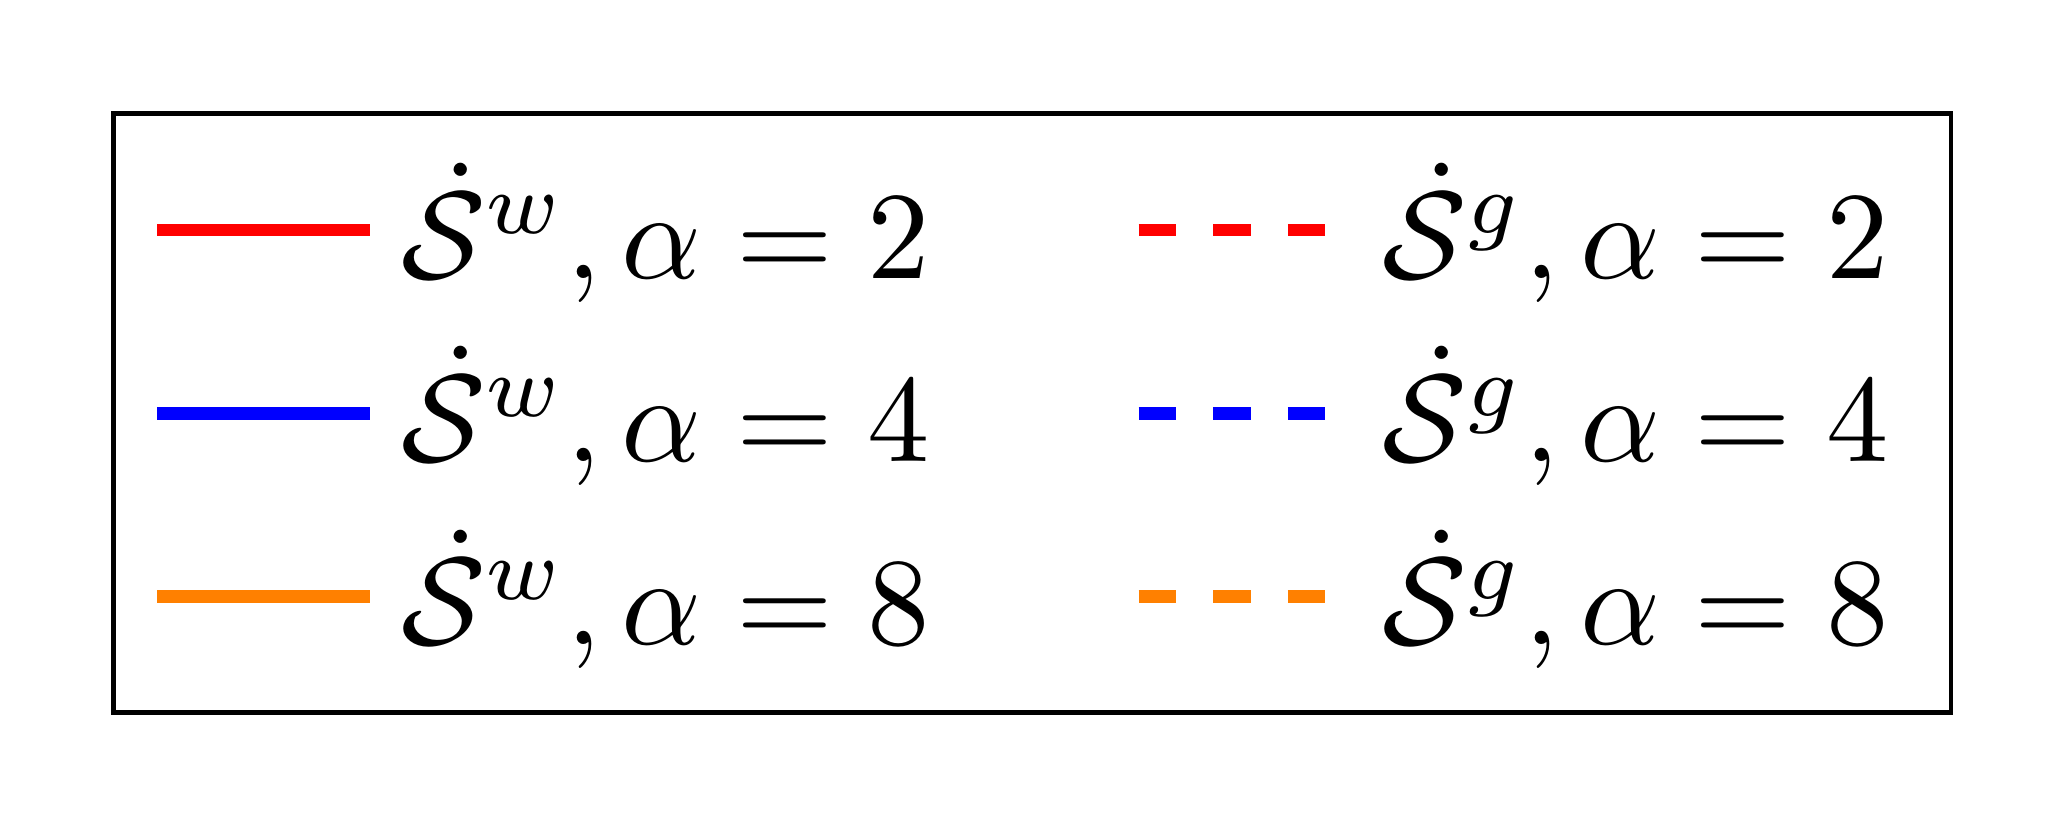
\includegraphics[width = 0.25\textwidth]{figures/waiting_room_entLegend.png}
\caption{\footnotesize Plots of $\entpp^w$ and $\entpp^g$ against $\gamma$ for different values of $\alpha$. Here we have set $\beta$ to unity and expressed $\gamma$ and $\alpha$ in multiples of $\beta$. Notice the different vertical scales. There is a zero of entropy production at $\gamma = \sqrt{\alpha}$ for both systems. $\entpp^w$ and $\entpp^g$ display qualitatively different behaviours in the limits as $\gamma \rightarrow 0$ and $\gamma \rightarrow \infty$.}
\label{fig:CG_waiting_room_entropy_prod}
\end{figure}

\subsubsection{Mechanism of Entropy Production}\label{subsection:mechanism-wating-room}

The dynamic entropy production of a continuous-time semi-Markov chain along non-equilibrium trajectories, $\entpp$ can be split into two contributions \cite{martinez2019inferring}

\begin{align}\label{entropy-split}
\entpp = \entpp_{\text{aff}} + \entpp_{\text{wtd}}.
\end{align}

$\entpp_{\text{aff}}$ results from what are called the cycle affinities of the system. If $\Gamma$ is the incidence graph of a semi-Markov chain, and $\mathcal{C}$ is a closed loop on $\Gamma$, then we define the cycle affinity, $\mathcal{A}_{\mathcal{C}}$, as

\begin{align}\label{cycle-affinity}
\mathcal{A}_{\mathcal{C}} = \log \prod_{(i\rightarrow j) \in \mathcal{C}} \frac{a_{ij}}{a_{ji}},
\end{align}

where $a_{ij}$ is the transition rate for $i \rightarrow j$ and we are are using the convention that $\log(\frac{0}{0}) = 0$. By dynamic reversibility, $a_{ij} > 0$ implies $a_{ji} > 0$, so $\mathcal{A}_{\mathcal{C}}$ is well-defined. Letting $r_{\mathcal{C}}$ be the rate at which the cycle $\mathcal{C}$ is observed in the long-time limit, we have \cite{van2022thermodynamic}

\begin{equation}
\entpp_{\text{aff}} = \sum_{\mathcal{C}} r_{\mathcal{C}}\mathcal{A}_{\mathcal{C}}
\end{equation}

$\entpp_{\text{wtd}}$ arises from asymmetric waiting-time distributions in semi-Markov systems. These waiting-time distributions carry information about the history of the system. For example, as the WR system transitions from $\ket{3}$ to $\ket{w}$, it enters the combination state

\begin{align}
\ket{w_3} = \frac{\beta}{\beta+\gamma}\ket{4} + \frac{\gamma}{\beta + \gamma}\ket{2},
\end{align}

which is distinct from the state $\ket{w_1}$ defined in (\ref{w1_comb_state}). The states $\ket{w_1}$ and $\ket{w_3}$ have different waiting-time distributions according to their time evolutions,

\begin{align}\label{w-evolutions}
\begin{split}
\ket{w_1(t)} &= \frac{1}{\alpha e^{-(\alpha + \gamma)t}+ \gamma e^{-(\beta + \gamma)t}}\left (\alpha e^{-(\alpha + \gamma)t}\ket{2} + \gamma e^{-(\beta + \gamma)t}\ket{4}\right) \\
\ket{w_3(t)} &= \frac{1}{\beta e^{-(\beta + \gamma)t} + \gamma e^{-(\alpha +\gamma)t}}\left (\gamma e^{-(\alpha + \gamma)t}\ket{2} + \beta e^{-(\beta + \gamma)}\ket{4} \right)
\end{split}
\end{align}

An observer viewing the process in reverse will observe state $\ket{w_3}$ when $\ket{w_1}$ occurs in the forward process. The distinct waiting-time distributions then give rise to entropy production which is captured in Eqns. (\ref{1to3_EP}) \& (\ref{3to1_EP}). In fact, $\entpp_{\text{wtd}}$ is the only contribution to the entropy production of the WR process. Cycles such as $\mathcal{C}_1 = \ket{1} \rightarrow \ket{w} \rightarrow \ket{1}$, which do not navigate the whole phase space, will not contribute to entropy production because they have zero cycle affinity. We have rates $\alpha + \gamma$ for the transition $\ket{1} \rightarrow \ket{w}$ and $\beta + \gamma$ for the transition $\ket{w} \rightarrow \ket{1}$, hence,

\begin{align}
\mathcal{A}_{\mathcal{C}_1} = \log \left( \frac{\alpha + \gamma}{\beta + \gamma}\frac{\beta + \gamma}{\alpha + \gamma}\right) = 0.
\end{align}

and likewise for any other cycle that does not explore the entire phase space. A similar calculation will show that in fact \textit{all} cycles of the WR system have zero affinity. The underlying physical intuition is that if a cycle includes an edge $(i \rightarrow j)$ then it necessarily includes the reversed edge $(j \rightarrow i)$. Hence, the forward and reverse trajectories include the same transitions, albeit in a different order. For the granular waiting room the situation is reversed.

Consider a clock-wise cycle of the granular system shown in Figure \ref{granular_fig}, beginning from $\ket{1}$ and making transitions
\begin{align}
\ket{1}\xrightarrow{} \ket{2}\xrightarrow{t_2} \ket{3}\xrightarrow{t_3} \ket{4}\xrightarrow{t_4} \ket{1},
\end{align}

where $t_i$ is the time spent occupying a state before transitioning away from it. The transition $\ket{1} \rightarrow \ket{2}$ occurs at $t=0$ and $\ket{4} \rightarrow \ket{1}$ at the final observation time $t = T$. In reverse time, the observed sequence of states is,

\begin{align}
\ket{1}\rightarrow\ket{4}\xrightarrow[]{t_4}\ket{3}\xrightarrow{t_3}\ket{2}\xrightarrow{t_2}\ket{1}.
\end{align}

In reverse time, the observed sequence of transitions is different, but the time interval spent in each state remains unchanged. Moreover, the waiting-time distribution for each state is independent of the particle's history. For these reasons, we have

\begin{align}
\entpp^g_{\text{wtd}} = 0
\end{align}

in the granular system. In summary, we have 

\begin{align}\label{ent-prod-mech}
\entpp^g = \entpp^g_{\text{aff}}, \; \; \entpp^w = \entpp^w_{\text{wtd}}.
\end{align}

We have already discussed how the quantitative behaviour of $\entpp^w$ is different from that of $\entpp^g$ as $\gamma$ is varied. Equation (\ref{ent-prod-mech}) shows that the two arise from completely separate mechanisms. Hence, coarse graining affects not only the degree of entropy production, but also its mechanism. 





% Since the Markov description of the granular waiting room is stable under time reversal, the waiting time in any state
